\articlehead{Only 22\% of Furries are Gay}{JM}{2013}

Every three weeks, the Londonfurs hold a meet in a City bar. The bar is closed to the public on Saturdays, so it's a private party.

Every three weeks, one or two hundred so furries turn up. And just about every three weeks, there is a new member of the bar staff boggling at the crowd.

I recently overheard a new bartender ask, ``So, are you all gay or something?''. And his furry customer responded, ``Yeah''.

(But he was wrong. We're not all gay. We're not even mostly gay.)

The bartender made a comment and a knowing face, as if the Furry Universal Gayness Theory explained everything, and the furry wandered off with his drinks. I thought of correcting the bartender as he shaped to serve next in line, but I figured that he probably wasn't interested in a short lesson on furry demographics. And besides, I was thirsty.

The truth is that about 22\% of furries are gay.\footnote{Source: furrypoll.com}

Furrypoll (formerly the Furry Survey):

\begin{itemize}
  \item Furrypoll is online-only, running since 2008.
  \item The number of annual respondents has varied between 3,000 and 10,000 with no significant change in results over that time.
  \item I'm counting gay furries as ones who are ``completely homosexual'' or ``mostly homosexual''.
  \item The International Anthropomorphic Research Project reports a slightly higher proportion of gay furries based on a smaller but comparable sample size (ref). Their numbers are slightly different because some of their surveys are collected at conventions. I discuss this effect further down in this article.
\end{itemize}

There is an [adjective][species] visualization of this data available here(ref).

\begin{wrapfigure}{l}{0.3\textwidth}
  \begin{center}
    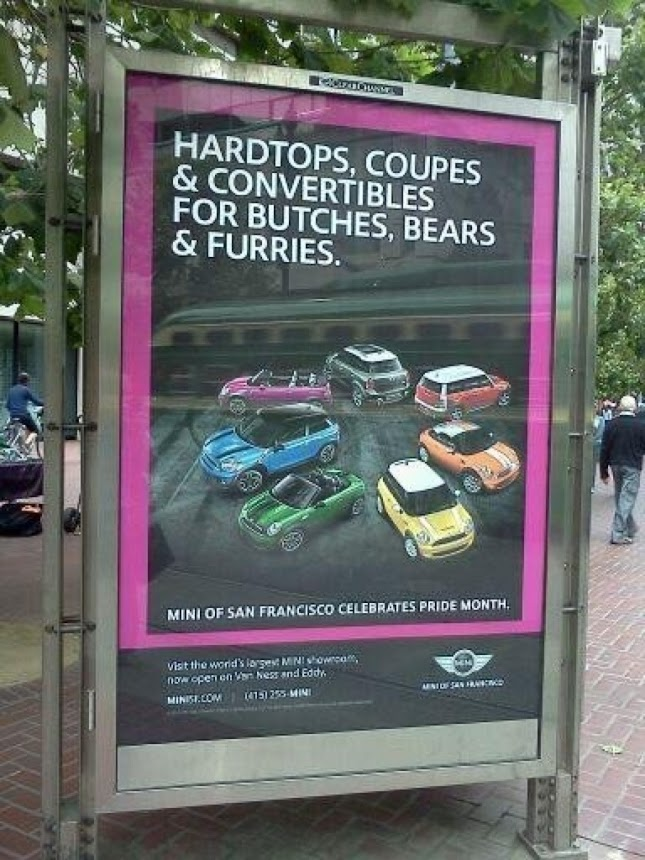
\includegraphics[width=0.25\textwidth]{content/assets/not-all-gay--mini}
  \end{center}
  \caption{Mini San Francisco billboard. It's interesting, but false: furry is not a queer phenomenon. Courtesy @fluff\_dragon.}
\end{wrapfigure}

The Furrypoll data on furry sexual preference is especially interesting if we look at how long the respondents have been part of the furry community. It shows that a lot of furries – an awful lot of furries – change their sexual preference, from straight to gay, within five years of joining the community.

\begin{figure}
  \begin{center}
    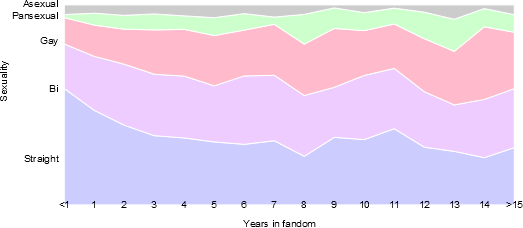
\includegraphics[width=\textwidth]{content/assets/not-all-gay--vis}
  \end{center}
  \caption{Years in the fandom vs. sexual orientation.}
\end{figure}

This shows that around 50\% of heterosexuals joining the furry community will change their sexual preference, mostly towards gay. I've written about this in detail before on [adjective][species], in an article titled Re-Evaluating Your Sexual Preference. The overall effect is that older furries are more likely to be gay.

Even with this large furry shift towards homosexuality over time, furry is still just 20 to 25\% gay. However we have a lot of furries who identify as bisexual, or at least in the bisexual area of the spectrum.

Bisexuality is a difficult term to define, because it tends to mean different things to different people. For some it means that gender is irrelevant to sexual attraction, others will swing between exclusively homosexual and heterosexual phases, and for others it merely denotes that the gender of their sexual or romantic partners is variable.

Because the meaning of `bisexual' is both reductive and variable, it's not very useful. This is a problem with a lot of terms associated with sexual orientation, gender, and identity. Unfortunately, when collecting data, we need to lump people into categories. Labelling a large portion of furry as `bisexual' is an unavoidable simplification.

I would argue that, inside furry, an unusually large proportion of our nominal bisexuals are people who are mostly heterosexual, but who enjoy homosexual sex. This occurs because homosexual (male) sex is highly available within furry: we are male dominated, sex-positive, and homosexual activity is normal.

In this way, furry neatly mirrors the non-furry world. In the non-furry world, nominal bisexuals are more likely to be mostly homosexual people who engage in heterosexual sex. This is because heterosexual sex is more available in the non-furry world; a product of a 50/50 gender split, a relative dearth of homosexuals, and cultural homophobia.

So furry encourages situational homosexuality, just like the non-furry world encourages situational heterosexuality. (As an aside, anyone using the term `jailhouse gay' to describe furries is being homophobic, because that term is only pejorative if you think that gay sex is `bad' compared to straight sex.)

The preponderance of gay sex within furry probably explains why real-world furry gatherings tend to be gayer than the community as a whole. A few things happen:

\begin{itemize}
  \item Gay furries are more likely to experience and enjoy sexual tension, real or imagined, at a furry gathering. This acts as a motivating factor.
  \item Straight furries who are in a relationship are less likely to have a partner who is also a furry. (Only about 20\% of furries are female.) And a furry with a non-furry partner is probably less likely to socialize with the group than an all-furry couple.
  \item Data shows that female furries are less likely than male furries to socialize in person (see below). The dearth of women means that there is less motivation for straight (male) furries to socialize. Women are less likely to socialize for two reasons: firstly, women tend to identify less strongly as a furry (ref furrypoll.com); secondly, women in the very male-dominated furry environment are often harassed (more on this in a moment).
\end{itemize}

You can see the differences by comparing furrypoll.com data, which is collected exclusively online, with International Anthropomorphic Research Project data, which is partly collected (45\%) in person at conventions.

\begin{itemize}
  \item Proportion of women: 20\% Furrypoll vs 15\% IARP
  \item Proportion of homosexuality: 22\% Furrypoll vs 29\% IARP
\end{itemize}

The differences would be starker still if the IARP data were 100\% from conventions.

As an aside, there is one group of furries with no doubt that there are a lot of heterosexuals at furry gatherings: women. It's common for women to be harassed, not necessarily in an overtly sexual fashion, but certainly in an unwelcome fashion. This is based on conversations I've had with women rather than any hard data: they tend to use terms like `annoying' and `pest' and `don't get the hint'. Some women choose to avoid furry gatherings altogether, which is bad for everyone.

Returning to the bar in London, it's easy to see how our furry reached the mistaken conclusion that we were ``all gay''. Men, and gay men, were over-represented. There were plenty of heterosexual men attending that Londonfurs meet, but they were largely invisible. Furries are often assumed to be gay (or bi) unless proven otherwise. This is another inversion of the real world: at furmeets, heterosexuality is always present but largely hidden. It's easy to draw the false conclusion that it doesn't exist.
